\section{Experiments}
\label{sec:experiments}

Experiments were conducted in the KITTI Road/Lane Dataset, part of KITTI Vision Benchmarking Suite~\cite{KITTI}. The dataset  contains  images for road and lane estimation for the task of image segmentation. It is consisted of 289 training and 290 test images. The ground-truth is manually annotated for two different road types: (i) road, road area composing all lanes; and (ii) lane, lane the vehicle is currently driving on. It is important to notice that the ground-truth is only available for training set and the test evaluation should be performed using KITTI Server.

In this work, it is used only the road ground-truths and the lane annotations were ignored. This dataset contains the same image with different ground-truths for lane and road estimation. Then, we prefer to use the road estimation and build the classifier on a binary problem~(road and background). The road type is divided in three different categories of road scenes, namely: (i) uu\_road, urban unmarked; (ii) um\_road, urban marked; and (ii) umm\_road, urban multiple marked lanes.  

To increase the number of images in the training set, it is performed some data augmentation procedures. The following techniques were made: pepper/salt noise, horizontal flipping (mirror), contrast change, brightness change, noise shadow and random rain/snow. Procedures that would create undesired behavior, such as the road in the sky and distortions that would change the nature of the objects in the scene, such as cars and pedestrians were avoided. Augmentation procedures resulted in 2601 images, divided in 2080 samples for training and 521 samples for validation (about 20\%). 


\subsection{Experimental setup}
   
Our networks were build using using Keras \cite{chollet2015keras} with Tensorflow \cite{tensorflow2015-whitepaper}. We used a pre-trained VGG16 model to initialize the weights. Also, we use SGD optimization with learning rate set to 1e-3, decay of 5e-6 and momentum of 0.95. The default batch size contains 16 images. All training experiments were performed in GeForce GTX 1080 8GB GPU.

For simplicity, in the remaining of this work, the network using the side outputs extracted at each stage of the VGG will be called Stage Layer Outputs~(\textbf{SLO}) and it is composed by $n=5$ side outputs. Similarly, for the side outputs extracted at each convolutional layer, it will be called All Layers Outputs~(\textbf{ALO}) and it is composed by $n=13$ side outputs. For comparison, it is also defined a network similar to VGG, with only the final output, without any side outputs, called No Side Outputs~(\textbf{NSO}).

The operations to combine side outputs are presented in the name of the methods. The merging operations \textbf{ADD}, \textbf{AVG} and \textbf{MAX} are available for both ALO and SLO methods. Once NSO does not contains side outputs, it does not contains merging strategies.

\subsection{Training results - Methods Comparison}

The first test set was design to identify the best neural network and its best merging methods. We train all nets with all merging methods for 100 epochs to determine which one learns faster and achieve the best results. This conduct lead us to understand how layers can be easily combined to produce outputs with good precision.

Figures \ref{fig:validation_accuracy_pixel_error} presents the relevant curves obtained during the training phase for the proposed approaches. Figure \ref{fig:validation_accuracy_pixel_error}, presents fuse pixel error loss for tested approaches. ALO networks appears to be more stable with a faster decay than NSO and all SLO approaches. Also, it is important to notice that NSO and SLO-MAX produces high instability in the learning course (SLO-MAX seens to overfitting around 40 epochs). By other hand, ALO-AVG presents the best result for the test, followed by ALO-MAX and ALO-ADD merging strategies.

\begin{figure}
  \caption{Categorical Cross-Entropy Validation Accuracy and Pixel Error Validation Loss}
  \centering
  %\begin{tabular}{ll}
    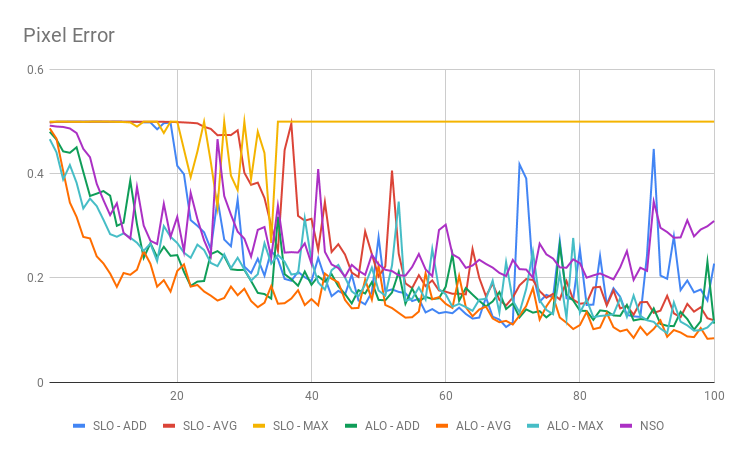
\includegraphics[width=1.\columnwidth]{figures/falreis/pixel_error.png}
  
    %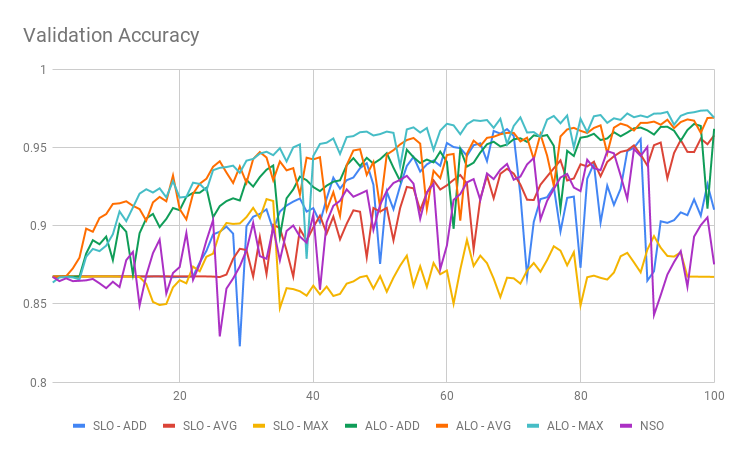
\includegraphics[width=1.\columnwidth]{figures/falreis/validation_accuracy.png}
  %\end{tabular}
  \label{fig:validation_accuracy_pixel_error}
\end{figure}

From previous graph, it is possible to conclude that ALO networks had superior and more desirable behavior than the SLO and NSO models. It is believed that these results are consequence of the considerably larger amount of side outputs, which create more possibilities of interchangeability between confident values.

\subsection{Best results}

In order to improve the results, a new set of tests were performed using 500 training epochs. As some networks had a poor performance in the previous test and other tests with different parameters, we decided to evaluated only ALO network in this new round of tests. The categorical cross entropy validation accuracy and pixel error validation loss for ALO nets are available in Figure \ref{fig:val_acc_500_epochs}.

\begin{figure*}
  \caption{Categorical Cross Entropy Validation Accuracy and Pixel Error Validation Loss results for 500 epochs test set}
  \centering
  \begin{tabular}{ll}
    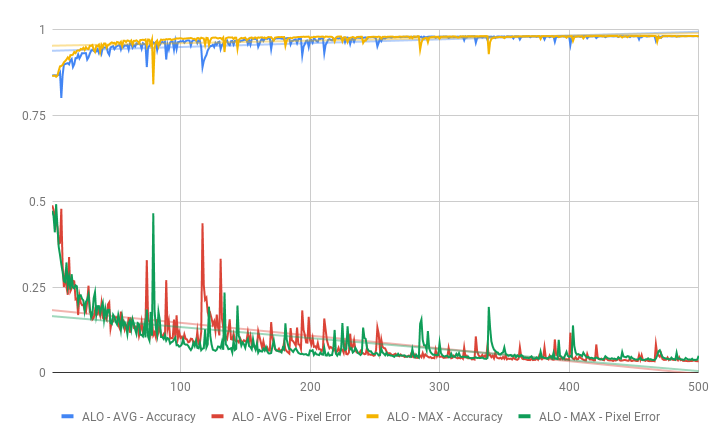
\includegraphics[width=1.\columnwidth]{figures/falreis/val_acc_500_epochs.png}
  
    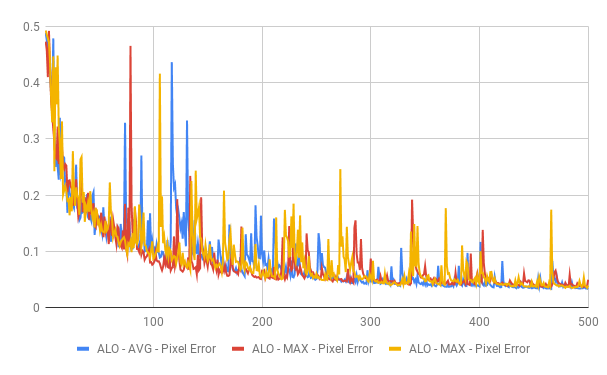
\includegraphics[width=1.\columnwidth]{figures/falreis/pixel_error_500_epochs.png}
  \end{tabular}%
  \label{fig:val_acc_500_epochs}
\end{figure*}

The best results of both metrics are quite similar for all networks. This indicates absence of a far better method to combine side outputs. The best result for cross entropy validation metric is just \textbf{0.0009} above the worst one (0.0332 for ALO-AVG and 0.0372 for ALO-MAX). For pixel-error validation loss, the best value is just \textbf{0.0040} above the worst one (0.983 for ALO-ADD and 0.9821 for ALO-AVG). {\color{red}Application of standard deviation to evaluate the stability of the methods also does not indicates a far away better method.}

Due to the similarity of the results, we will indicate the best method using the value of validation pixel-error loss metric. For this criteria, ALO-AVG was defined as the best method of our training set.

\subsection{Post-processing using mathematical morphology}

After the training procedure, we create a post processing step to reduce possible noises in results proposition. For this, we used the mathematical morphology operation of Opening~\cite{najman13}. This procedure removes small noises created by the foreground~(the road) in the background. We defined a set of kernels with the sizes of $5\times5$, $7\times7$, $9\times9$, $11\times11$ and $13\times13$ and applied in the images to reduce different sizes of noises. 

A simple comparison is presented in Figure \ref{fig:post_processing_comp}. In this image, we selected an output result that clearly shows the benefits of mathematical morphology post processing. It is possible to see the removal of part of the noise in the far right of the image (\textit{white pixels}). This procedure increase the confidence, once small variations in the results can lead a potential problem, if used in a self-driving vehicle. 

A negative interference of this method is the removal of some points that seens to fit correctly. This situation happens frequently in the base of the road proposition. In Figure \ref{fig:post_processing_comp}, it can be seen in the botton left and the bottom right of the road (\textit{red pixels}).

\begin{figure}
  \caption{Comparison between ALO-AVG without post processing and ALO-AVG with post-processing with mathematical morphology. In the last picture, \textit{white} pixels represents desirable differences while \textit{red} pixels represents undesirable ones.}
  \centering
  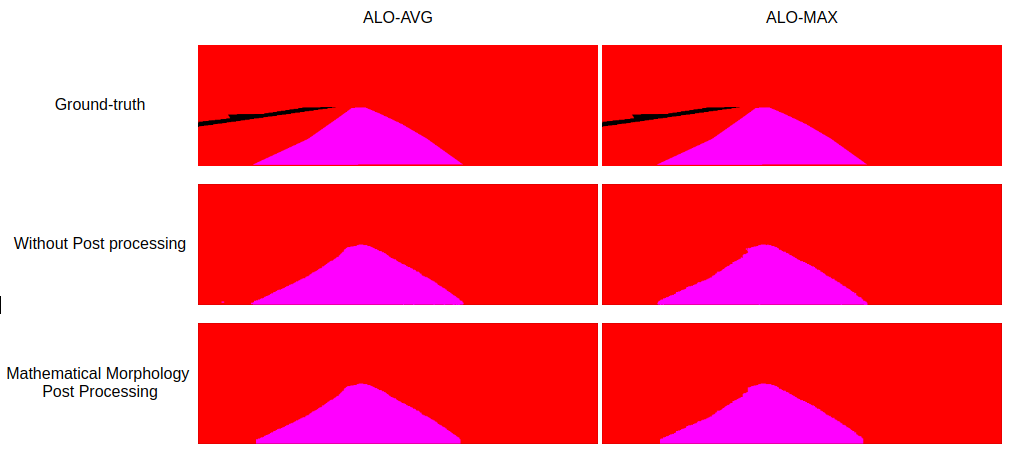
\includegraphics[width=1.\columnwidth]{figures/falreis/post_processing_comparison.png}
  \label{fig:post_processing_comp}
\end{figure}

\subsection{Evaluation results and comparison with the state-of-the-art}

Reminding that the test evaluation could only be performed using KITTI Server, the metrics provided are maximum F1-measure~(MaxF), average precision~(AP), precision~(PRE), recall~(REC), false positive rate~(FPR) and false negative rate~(FNR). 

The server tests were performed using ALO-AVG method, the best one in the training process. To provide succint labels, we will use the name \textbf{ALO-AVG} for the regular approach and \textbf{ALO-AVG-MM} for the version with mathematical morphology post-processing. 

The results achieved  on the test set according to each category in the road scenes are presented in Table~\ref{tab:metrics}. As expected, the ALO-AVG-MM model performed better then the ALO-AVG in all almost all of the cases. {\color{red}It is also possible to notice that although the post-processing slightly improved the overall performance, it also increased the number of false negatives. This could be an indications that perhaps the applied kernel sizes are not adequate and are removing more of the foreground than the desired.}

If compared with the state-of-the-art~(called \textit{PLARD}, an anonymous submission on the KITTI Server platform), the proposed method is comparable and sometimes superior, regarding the maximum F1-measure and the recall metrics. This is due the fact that although the reported state-of-the-art on the dataset presents a superior average precision, it also almost always presents a higher rate of false positives an negatives. This indicates that the proposed methods are more precise in delineating the regions to be segmented.

\begin{table}
 \scriptsize
 \caption{KITTI benchmark evaluation results for each category}
  \begin{tabular}{{l}{c}{c}{c}{c}{c}{c}}
  
   \multicolumn{7}{l}{\textbf{um\_road}} \\
  \hline 
    Method & MaxF & AP & PRE & REC & FPR & FNR \\
  \hline
    \textit{SLO} & 96.92\% & 87.36\% & 94.47\% & \textbf{99.49\%} & 1.13\% & \textbf{0.51\%} \\
    \textit{SLO-mm} & \textbf{97.01}\% & \textbf{87.68\%} & \textbf{94.83\%} & 99.30\% & \textbf{1.05\%} & 0.70\% \\
    \textit{ALO}  & 96.39\% & 86.81\% & 93.87\% & 99.05\% & 1.25\% & 0.95\% \\
    \textit{ALO-mm} & 96.65\% & 87.51\% & 94.64\% & 98.74\% & 1.08\% & 1.26\% \\
    \textit{State-of-the-art} & \textbf{97.05\%}& \textbf{93.53\%} &\textbf{97.18\%} &\textbf{96.92\%} &	\textbf{1.28\%} &\textbf{3.08\%} \\
  \hline
  \multicolumn{7}{c}{} \\
  
  \multicolumn{7}{l}{\textbf{umm\_road}} \\
  \hline 
    Method & MaxF & AP & PRE & REC & FPR & FNR \\
  \hline
    \textit{SLO}  & 97.57\% & 89.44\% & 96.05\% & \textbf{99.15\%} & 1.24\% & \textbf{0.85\%} \\
    \textit{SLO-mm} & \textbf{97.61\%} & \textbf{89.67\%} & \textbf{96.30\%} & 98.97\% & \textbf{1.16\%} & 1.03\% \\
    \textit{ALO}  & 97.05\% & 88.83\% & 95.37\% & 98.78\% & 1.46\% & 1.22\% \\
    \textit{ALO-mm} & 97.21\% & 89.31\% & 95.90\% & 98.56\% & 1.29\% & 1.44\% \\
    \textit{State-of-the-art} & \textbf{97.77}\%&\textbf{ 95.64\%} &\textbf{97.75\%} &\textbf{97.79\%} &	\textbf{2.48\%} &\textbf{2.21\%} \\
  \hline
  \multicolumn{7}{c}{} \\
  
  \multicolumn{7}{l}{\textbf{uu\_road}} \\
  \hline 
    Method & MaxF & AP & PRE & REC & FPR & FNR \\
  \hline
    \textit{SLO}   & 95.16\% & \textbf{85.73\%} & 92.94\% & 97.49\% & 1.16\% & 2.51\% \\
    \textit{SLO-mm}  & \textbf{95.42\%} & 86.48\% & \textbf{93.77\%} & 97.13\% & \textbf{1.01\%} & 2.87\% \\
    \textit{ALO}   & 94.70\% & 84.87\% & 92.00\% & \textbf{97.56\%} & 1.33\% & \textbf{2.44\%} \\
    \textit{ALO-mm} & 95.20\% & 86.15\% & 93.40\% & 97.08\% & 1.08\% & 2.92\% \\
    \textit{State-of-the-art} & \textbf{95.95\%}& \textbf{95.25\%} &9\textbf{5.25\%} &\textbf{95.65\%} &	\textbf{1.21\%} &\textbf{4.35\%} \\
  \hline
  \multicolumn{7}{c}{} \\
  \end{tabular} 
  \label{tab:metrics}
\end{table}


As a final and visual representation of the results, we presents in Figure \ref{fig:visual_representation}. This image shows the results marked (in green) over the road, to shows the performance of our model.

\begin{figure}
  \caption{Visual representation of the results}
  \centering
  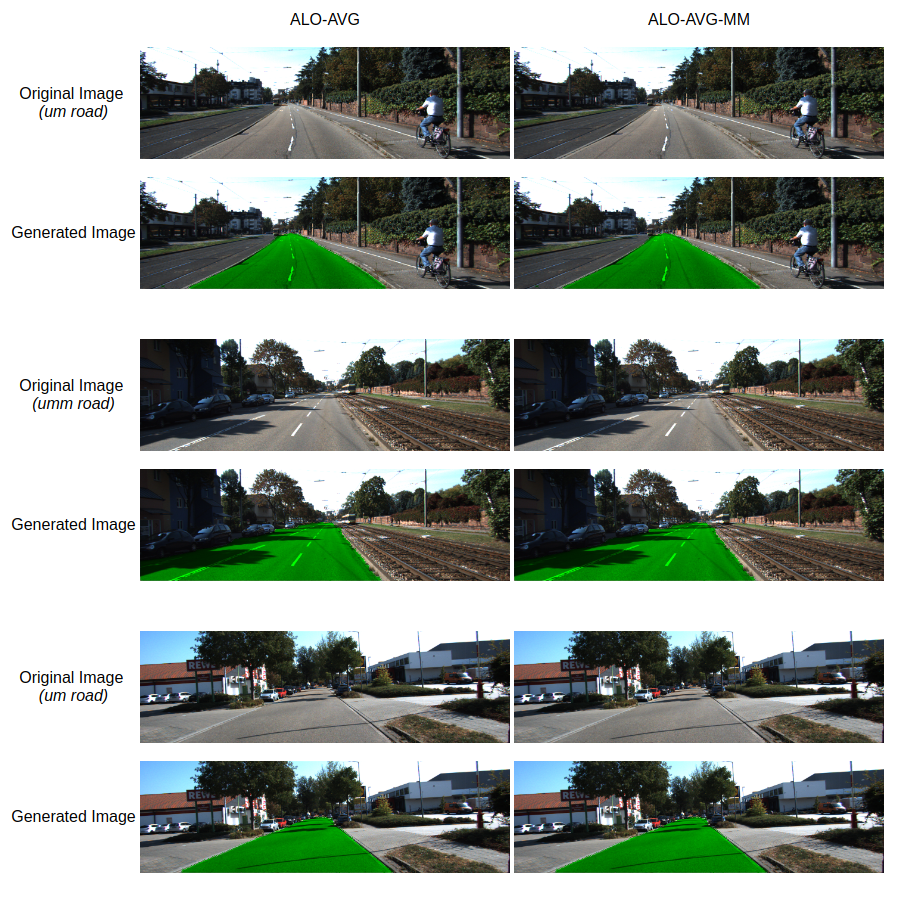
\includegraphics[width=1.\columnwidth]{figures/falreis/visual_representation.png}
  \label{fig:visual_representation}
\end{figure}
